
\subsection{Regelstrecke}
In der Regelungstechnik wird die zu regelnde Strecke als Regelstrecke bezeichnet. Die Regelstrecke wird durch ihr Zeitverhalten charakterisiert, welches den Aufwand und die Güte der Regelung bestimmt. Um das Zeitverhalten zu beschreiben verwendet man die Sprungantwort, welche zeigt, wie die Regelgrösse auf Stellgrössenänderung reagiert. Mit der entstehenden Regelgrösse werden verschiedene Regelstrecken unterschieden:
\begin{itemize}   
 \item  P-Regelstrecke
 \item I-Regelstrecke
 \item    Strecken mit einer Totzeit
 \item Strecken mit Energiespeicher
\end{itemize}

Dieses Projekt beschäftigt sich mit  den PTn-Strecken, welche eine Kombination aus einer Strecke mit proportionalen Verhalten und einer mit Totzeit sowie der Angabe der  Ordnung n der Strecke.

\subsubsection*{P-Regelstrecke}
Bei der Regelstrecke mit proportionalem Verhalten folgt die Regelstrecke proportional der Stellgrösse ohne Verzögerung. Dies kommt in der Praxis nicht vor, da immer eine Verzögerung vorhanden ist. Ist diese jedoch sehr klein spricht man von einer P-Strecke. Das Verhalten der Strecke ist in seinem Blockschaltbild (Abb.\ref {fig:PStrecke}) symbolisch dargestellt. Der Proportionalitätsfaktor wird mit $K_p$ abgekürzt. Wird $K_p<1$ wirkt $K_p$ nicht mehr verstärkend sondern abschwächend.\\
\todo{Bild Blockschaltbild P-Strecke}
\begin{figure}[h!, width=\pagewidth]
\begin{center}
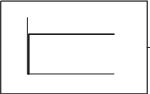
\includegraphics[width=0.2\textwidth]{images/PStrecke}
\caption{Blockschaltbild von P-Strecke}
\label{fig:PStrecke}
\end{center}
\end{figure}


\subsubsection*{Strecken mit Totzeit}
Ändert sich die Stellgrösse, wirkt sich diese Änderung bei einer Strecke mit Totzeit erst nach einer gewissen Zeit auf die Regelgrösse aus. Mit $T_t$ wird das Mass der Totzeit gekennzeichnet.
Totzeiten verursachen schnell Schwingungen, da sich die Stellgrösseänderung zeitverzögert auf die Regelgrösse auswirkt. Die Schwingungen entstehen wenn sich die Stellgrösse und die Regelgrösse periodisch ändern.
\begin{figure}[h!, width=\pagewidth]
\begin{center}
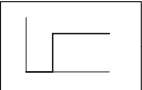
\includegraphics[width=0.2\textwidth]{images/TotZeit}
\caption{Blockschaltbild von Strecke mit Totzeit}
\label{fig:TotZeit}
\end{center}
\end{figure}


\subsubsection*{I-Regelstrecke}
Die I-Regelstrecke antwortet auf eine Stellgrössenänderung mit einer fortwährenden 
Änderung in steigende oder fallende Richtung. Die Begrenzung dieses Vorganges ist mit den systemgegeben Schranken gegeben. Die Integrierzeit $T_i$ ist ein Mass für die Anstiegsgeschwindigkeit der Regelgrösse und das Blockschaltbild (Abb. \ref{fig:IStrecke}) zeigt das Verhalten sinnbildlich.

\begin{figure}[h!, width=\pagewidth]
\begin{center}
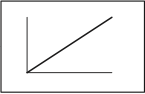
\includegraphics[width=0.2\textwidth]{images/IStrecke}
\caption{Blockschaltbild von I-Strecke}
\label{fig:IStrecke}
\end{center}
\end{figure}


\subsection{Regler}
Die Aufgabe eines Reglers besteht die zu regelnde Strecke mit einem Stellsignal so zu beeinflussen, dass der Wert der Regelgrösse gleich dem Wert der Führungsgrösse entspricht. Der Regler besteht aus einem Vergleichsglied, welches die Reglerdifferenz aus der Differenz zwischen Führungs- und Reglergrösse bildet und dem Reglerglied. Das Reglerglied erzeugt aus der Reglerdifferenz die Stellgrösse.
Es wird zwischen P-, I- und D-Regler unterschieden.\\
In diesem Projekt werden die PI- und PID-Regler, welche Kombinationen der oben genannten Regler sind, behandelt.\\

\subsubsection{PI-Regler}
Der PI-Regler besteht aus einer Parallelschaltung von einem P- und einem I-Regler (Abb.\ref{fig:PIRegler}). Durch diese Kombination werden die Nachteile beider Regler aufgehoben und die Vorteile (schnell, stabil) hervorgehoben. Sein Verhalten wird bildlich in dem Blockschaltbild in Abbildung \ref{fig:PIRegler2}.\\

\begin{figure}[h!, width=\pagewidth]
\begin{center}
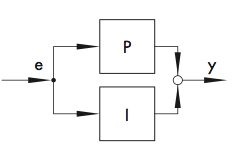
\includegraphics[width=0.4\textwidth]{images/PIRegler1}
\caption{Parallelschlatung von P-Regler und I-Regler}
\label{fig:PIRegler1}
\end{center}
\end{figure}

\begin{figure}[h!, width=\pagewidth]
\begin{center}
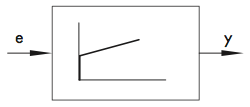
\includegraphics[width=0.4\textwidth]{images/PIRegler2}
\caption{Blockschaltbild von PI-Regler}
\label{fig:PIRegler2}
\end{center}
\end{figure}


\subsubsection{PID-Regler}
Wird dem PI-Regler ein D-Anteil parallel geschaltet (Abb. \ref{fig:PRDRegler}), entsteht der PID-Regler. Der PID-Regler ist ein sehr oft verwendeter Regler, da durch den D-Anteil die Regelgrösse rascher den Sollwert erreicht und der Einschwingvorgang schneller abgeschlossen ist. Das Blockschaltbild zeigt dieses Verhalten (Abb.\ref{fig:PIDRegler2}) figürlich. Der PID-Regler ist geeignet für Strecken höheren Ordnungen, welche möglichst schnell und ohne bleibende Regelabweichung geregelt werden müssen.

\begin{figure}[h!, width=\pagewidth]
\begin{center}
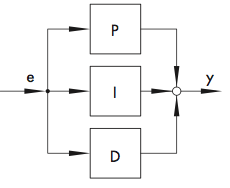
\includegraphics[width=0.4\textwidth]{images/PRDRegler1}
\caption{Parallelschaltung von P-, I-, und D-Regler}
\label{fig:PRDRegler1}
\end{center}
\end{figure}

\begin{figure}[h!, width=\pagewidth]
\begin{center}
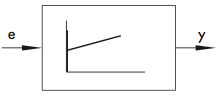
\includegraphics[width=0.4\textwidth]{images/PIDRegler2}
\caption{Blockschaltbild des PID-Reglers}
\label{fig:PIDRegler2}
\end{center}
\end{figure}


\subsection{Die Steuerung}

Unter einer Steuerung versteht man eine offen Wirkungskette wie in Abbildung \ref{fig:Steuerung}, dass heisst die Wirkglieder sind kettenähnlich aufgereiht und besitzen keine Rückkopplung. Die Steuerkette wird genau für eine Steuerung ausgelegt und kann nur einer Störgrösseart entgegenwirken. Ohne die Rückkopplung wird das Ausgangsignal nicht mit dem Eingangssignal verglichen und es können keine Korrekturen vorgenommen werden.

\begin{figure}[!h!, width=\pagewidth]
\begin{center}
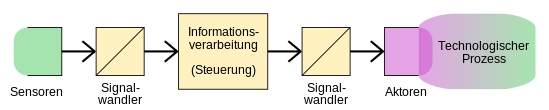
\includegraphics[width=0.5\textwidth]{images/Steuerung}
\caption{Steuerung}
\label{fig:Steuerung}
\end{center}
\end{figure}

\subsection{Der geschlossene Regelkreis}
Die Aufgabe eines geschlossenen Regelkreises (Abbildung \ref{fig:geschlossenerRegelkreis}) ist es, einen vorgegeben Sollwert zu erreichen und diesen
auch bei St\"orungen aufrecht zu erhalten. Dabei sollen die unten genannten
dynamischen Anforderungen eingehalten werden, damit die Stabilit\"at des
Regelsystems garantiert ist. Die wichtigste Bedingung f\"ur die Schrittantwort
ein geschlossenen Regelkreis heisst, dass der Regelfehler, die Differenz
zwischen Ist- und Sollwert, gleich Null oder m\"oglichst klein ist.\\


\begin{figure}[!h!, width=\pagewidth]
\begin{center}
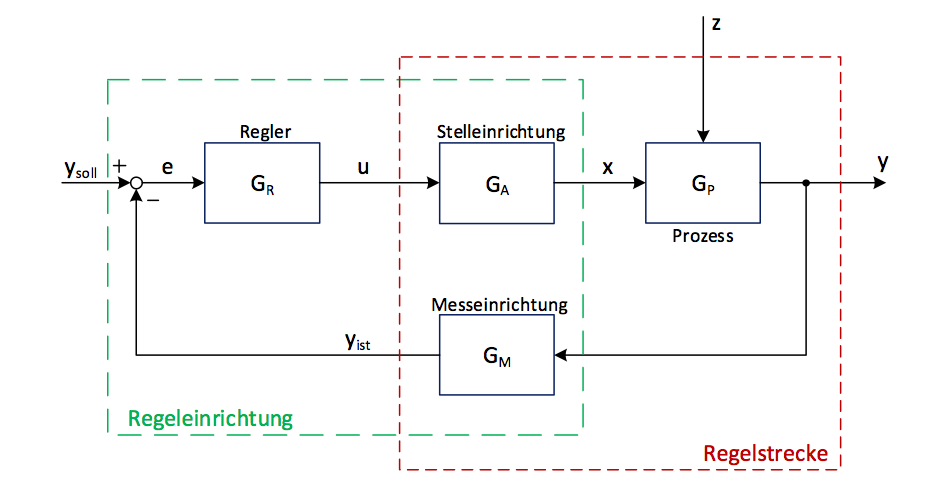
\includegraphics[width=0.5\textwidth]{images/geschlRegelkreis}
\caption{Geschlossener Regelkreis}
\label{fig:geschlossenerRegelkreis}
\end{center}
\end{figure}

%Name Bild Struktur eines allgemeinen Regelkreises
\begin{itemize}
\item
$y_soll$ bezeichnet den Sollwert der Regelgr\"osse.
\item
$e$ Regelabweichung (Regelfehler)
\item
$u$ Steuergr\"osse
\item
$x$ Stellgr\"osse
\item
$y$ Regelgr\"osse
\item
$z$ St\"orgr\"ossen werden in diesem Projekt nicht berücksichtigt
\item
$y_ist$ ist der Ist-Wert der Regelgr\"osse und wird auch als die
Schrittantwort des Regelkreises bezeichnet.
\end{itemize}


Grunds\"atzlich k\"onnen f\"unf Anforderungen f\"ur einen geschlossenen
Regelkreis und deren Schrittantworten zusammengefasst werden:\\
\begin{enumerate}
\item Der Regelkreis muss stabil sein:\\
F\"ur das Regelsystem heisst stabil, dass es in seinen
Gleichgewichtszustand zur\"uckgef\"uhrt werden kann.
\item
Der Regelkreis muss gen\"ugend ged\"ampft sein.
\item
Der Regelkreis muss eine bestimmte station\"are Genauigkeit
aufweisen: \\Das bedeutet, der Regelfehler e(t) soll f\"ur t-> oo
gegen Null gehen. 
\item
Der Regelkreis muss hinreichend schnell sein: 
Ist die D\"ampfung zu stark oder zu schwach, braucht der
Einschwingvorgang mehr Zeit. Hierbei muss darauf geachtet werden, dass
die spezifischen Anforderungen an das Regelsystem eingehalten werden.
\item
Der Regelkreis muss robust sein: Der Regelkreis muss so ausgelegt
werden, dass das Regelsystem auch im schlimmsten Fall (je nach
Regelsystem situationsabh\"angig) in der Lage ist, das System zur\"uck
in den stabilen Zustand (vgl. 1.) zu regeln.
\end{enumerate}

\subsubsection{Die Schrittantwort des geschlossenen Regelkreises}
\todo{Bild Schrittantworten passend zu Aufzählung unten}

Als Schrittantwort eines geschlossenen Regelkreises wird das Ausgangssignal y(t) bezeichnet. Im Zusammenhang mit den Anforderungen an den geschlossenen Regelkreis, werden an die Schrittantwort folgende Forderungen gestellt:
\begin{enumerate}
\item
Die Schrittantwort eines stabilen Regelkreises darf nach dem Erreichen
des eingeschwungenen Zustand kein erneutes \"Uberschwingen auftreten.

\item
Die D\"ampfung der
Schrittantwort soll so stark sein, dass der eingeschwungene Zustand
m\"oglichst rasch erreicht wird ohne dass das \"Uberschwingen des
Systems zu stark wird.
\item Die Schrittantwort muss für ein $t\rightarrow\infty$ gleich $y_{soll}$ sein.
\item Die Schnelligkeit des
Einschwingvorganges der Schrittantwort ist stark von der D\"ampfung
abh\"angig. Wenn diese zu stark oder zu schwach ist, ist der Regelkreis zu langsam.
\end{enumerate}
